\documentclass{article}

\usepackage[english]{babel}
\usepackage[utf8]{inputenc}
\usepackage{amsmath,amssymb}
\usepackage{parskip}
\usepackage{graphicx}
\usepackage{subfigure}
\usepackage{hyperref}
\usepackage{algorithm}
\usepackage{algpseudocode}
\usepackage{multirow}
\usepackage{float}
%\usepackage{algorithmicx}

% Margins
\usepackage[top=2.5cm, left=3cm, right=3cm, bottom=4.0cm]{geometry}

% custom footers and headers
\usepackage{fancyhdr}
\pagestyle{fancy}
\lhead{}
\chead{}
\rhead{}
\lfoot{}
\cfoot{}
\rfoot{Page \thepage}
\renewcommand{\headrulewidth}{0pt}
\renewcommand{\footrulewidth}{0pt}


\usepackage{multicol}
\usepackage{tikz}

% code listing settings
\usepackage{listings}
\usepackage{xcolor}

\definecolor{codegreen}{rgb}{0,0.6,0}
\definecolor{codegray}{rgb}{0.5,0.5,0.5}
\definecolor{codepurple}{rgb}{0.58,0,0.82}
\definecolor{backcolour}{rgb}{0.95,0.95,0.92}
\definecolor{framecolour}{rgb}{0.81,0.81,0.77}

\lstdefinestyle{mystyle}{
    aboveskip={1.0\baselineskip},
    belowskip={1.0\baselineskip},
    backgroundcolor=\color{backcolour},   
    commentstyle=\color{codegreen},
    keywordstyle=\color[rgb]{0.627,0.126,0.941},
    numberstyle=\tiny\color{codegray},
    stringstyle=\color{codepurple},
    basicstyle=\ttfamily\footnotesize,
    %numbers=left,
    frame=single,
    rulecolor=\color{framecolour},
    breakatwhitespace=false,         
    breaklines=true,                 
    captionpos=b,                    
    keepspaces=true,                 
    numbersep=5pt,                  
    showspaces=false,                
    showstringspaces=false,
    showtabs=false,                  
    tabsize=2
}

\lstset{style=mystyle}


%%%%%%%%%%%%%%%%%
%     Title     %
%%%%%%%%%%%%%%%%%
\title{Final report \\ Knowledge distillation for echocardiogram view classification}
\author{
  Andris Freimanis\\
  \texttt{gusandrifr@student.gu.se}
  \and
  Moritz Sprenger\\
  \texttt{gussprmo@student.gu.se}
  \and
  Raouf Bahsoun\\
  \texttt{gusbahsra@student.gu.se}
  \and
  Yu-Ping Hsu\\
  \texttt{gushsuyu@student.gu.se}
}
\date{\today \endgraf\bigskip\vspace*{12cm}
	\textbf{Supervisors}\\
	\centering Yinan Yu, academic supervisor, yinan@chalmers.se \\
	Charlotte von Numers, industry supervisor, charlotte.vonnumers@astrazeneca.com \\
	Luis Arevalo, industry supervisor, imarevost@gmail.com}



\begin{document}
\maketitle

%%%%%%%%%%%%%%%%%
%   Problem 1   %
%%%%%%%%%%%%%%%%%
\newpage
\tableofcontents
\newpage
\section{Abstract}

The heart is responsible for promoting blood circulation, transporting oxygen and nutrients to various organs and tissues of the body, as well as carrying away waste and carbon dioxide from the body. Having a normal ejection fraction value is vital for human health. Echocardiography is the most common method of measuring ejection fraction but it is highly dependent on correct execution by the practitioner to get the desired views for diagnostic purposes. Four different ultrasound views are classified using four different model architectures. Knowledge distillation methods are used to extract the knowledge from an existing VGG16 model and transfer it to small student models. The purpose of this project is to find an optimal student model with high accuracy, fast classification speed, and small model size so that it can perform optimally on mobile devices to help classify views and guide the correct image scanning. The four student models studied are Mobilenet-V3-small, Mobilenet-V3-large, Shufflenet, and Ghostnet. The results show that MobileNet-V3-large had the highest relative validation accuracy at 0.98. MobileNet-V3-small and ShuffleNet, are two smaller models and can achieve slightly higher inference speedups of 1.4.

\section{Introduction}
The heart is the key organ that maintains the normal operation of various functions of the human body. It controls the flow of blood. Without blood which supplies nutrients, organs, tissues or cells in the body are unable to continue working normally. The heart is located on the left side of the human chest and is divided into two parts, the left heart and the right heart. This division prevents the heart from mixing deoxygenated blood and oxygenated blood. Oxygenated blood is pumped by the left side of the heart, proceeds to systemic circulation via the aorta, and travels to various parts of the body to supply cell nutrients. After returning to the right atrium, it becomes hypoxic blood and travels to the lungs through the pulmonary artery to get oxygen. The oxygen-rich blood returns from the pulmonary veins to the left atrium, completing the pulmonary circulation and preparing for the next round of systemic circulation. The heart is like an electric pump, pumping blood throughout the body. The power of the pump mainly relies on the sinoatrial node located in the right atrium to send electrical signals to stimulate the contraction of myocardial tissue to generate heartbeats. Each heartbeat is a contraction and relaxation of the heart. The heart muscle contracts and relaxes regularly with each beat of the heart. When the heart contracts, blood is pumped from the left ventricle to the rest of the body. At the same time, the heart valves close to prevent blood from flowing backward. During relaxing, the valves open to allow blood to flow into and fill the ventricles in preparation for the next contraction. Ejection fraction is the percentage of blood pumped out of the heart each time it beats. 

A healthy human heart can only pump half to two-thirds of the blood from the left ventricle with each contraction. This means the normal ejection fraction is not 100\% for a healthy person. The normal ejection fraction is between 55\% and 65\%. The JACC: Heart Failure published in August 2022 reveals the impact of abnormal left atrial ejection fraction on the heart. Values that are too high or too low will increase the hazard ratio of major adverse cardiovascular events. 
The ejection fraction can be measured by the following method: (1) Echocardiography: Echocardiography, known as cardiac ultrasound, uses sound waves to create images of the heart's beating. These images show how blood flows through the heart and its valves. (2) Cardiac magnetic resonance imaging (MRI): It uses magnetic fields, radio waves, and a computer to create transverse images of the heart. (3) Cardiac computed tomography (CT) scan: X-rays from different angles are used to construct images of the heart. (4) Nuclear medicine scan: During a cardiac nuclear medicine scan, a small amount of radioactive material is injected into the bloodstream through a vein. Single photon emission CT/CT (SPECT/CT) and positron emission tomography/CT (PET/CT) cameras are used to track the radioactive material in the blood as it flows through the heart and lungs. Because cardiac images from MRI, CT, and nuclear medicine are all static, echocardiography is the most common method of measuring ejection fraction \cite{shah2022supranormal}. 

The basic principle of cardiac ultrasound uses the pulse-echo principle. The ultrasound transducer converts electrical signals into ultrasonic pulses. The pulse passes through the skin and into the internal anatomy at different speeds. When the ultrasonic sound waves encounter two different tissues with different characters or densities, the wave reflects. This phenomenon is called ultrasound reflection. The transducer receives the returning echoes and converts them to electric signals which a computer converts into points of brightness on the image corresponding to the anatomic position and the strength of the reflecting echoes. A complete image frame formed by ultrasound is called a sonogram. When a patient is diagnosed by ultrasound, many sonograms will be reconstructed into a video. 


The limitation of cardiac ultrasound is that the ultrasound wave will be obstructed by air or bones and cannot obtain clear images. For some patients with chest wall abnormalities, emphysema, or obesity, it is hard to sample images with good resolution. This makes diagnosis difficult. Cardiac ultrasound is an examination that highly relies on technology and experience. Providing a machine learning model on a mobile device or the medical equipment, that helps classify these views, could assist and guide operators in sampling correct images. This would greatly improve the imaging quality and further assist doctors in more accurate measurements of left ventricular ejection fraction. This way, the hidden dangers of the patient’s heart can be detected earlier, or the effectiveness of the patient’s heart treatment can be measured more accurately. 


The purpose of this project is to use knowledge distillation to transfer the knowledge of an existing teacher model to a student model and find an optimal student model with high accuracy, fast classification speed, and small model size so that it can perform optimally on mobile devices, for instance on a Raspberry Pi computer, given the requirement of being able to produce a video at 30 frames per second and having a memory size of less than $ 50 $ Megabytes.


\section{Literature Review}
Knowledge distillation (KD) denotes a method where a smaller student model is supervised by a larger teacher model and was popularized by \cite{hintonDistillingKnowledgeNeural2015}. The idea behind KD is that the student model mimics the teacher model and reaches similar or even greater performance with less capacity \cite{gouKnowledgeDistillationSurvey2021}. Figure \ref{fig:kd} shows the general setup for knowledge distillation methods. Both models are trained with the same data and the student network is supported by knowledge transferred from the teacher model.

\begin{figure}[htb]
	\begin{center}
		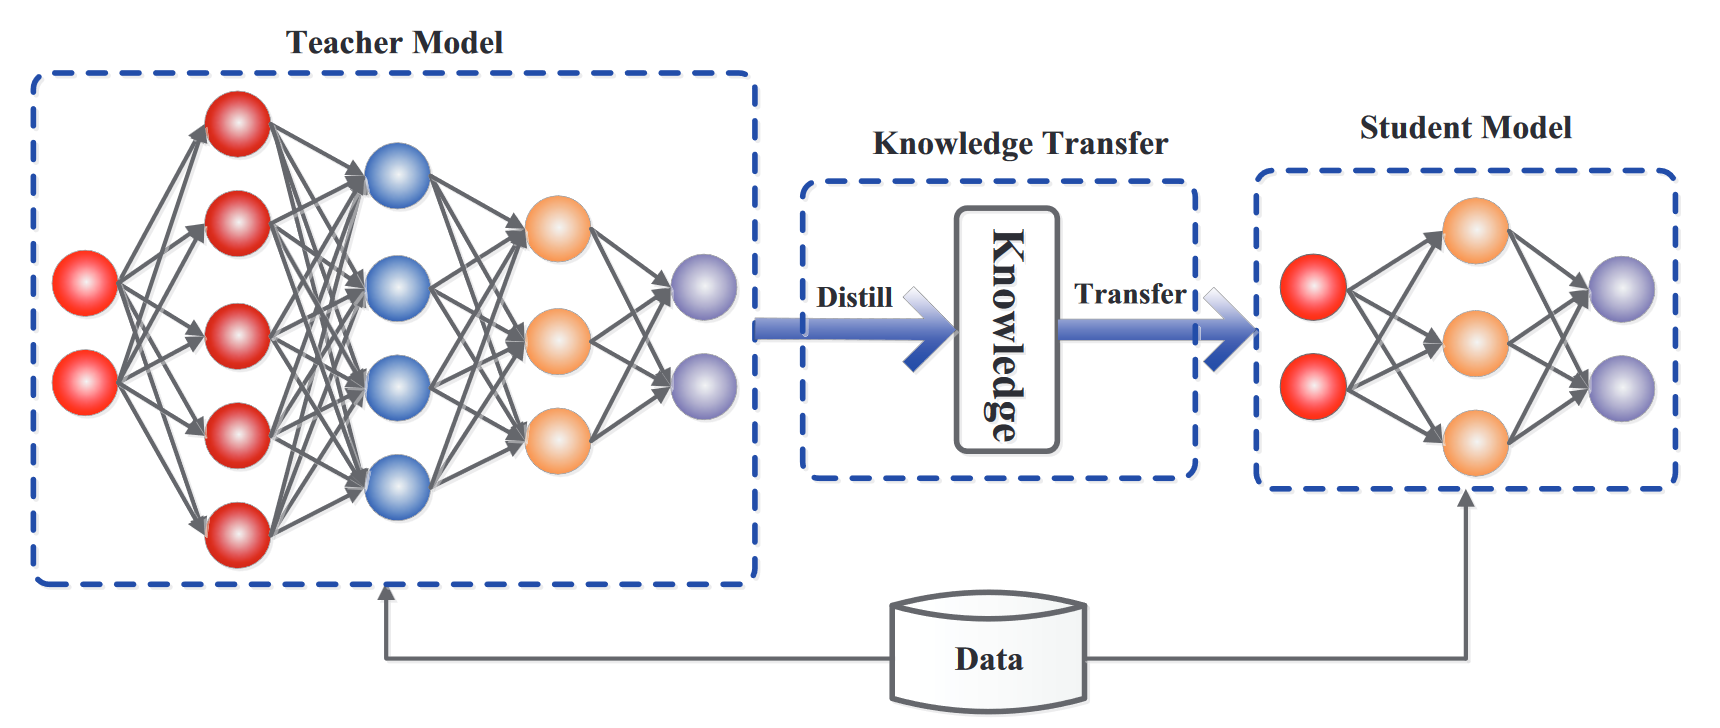
\includegraphics[width=150mm]{assets/kd}
	\end{center}
	\caption{Basic framework for knowledge distillation \cite{gouKnowledgeDistillationSurvey2021}}
	\label{fig:kd}
\end{figure}

Knowledge distillation system can generally be differentiated by their three main components: the type of knowledge, the distillation algorithm and the teacher-student architecture \cite{gouKnowledgeDistillationSurvey2021}.

Three main categories of knowledge are used to describe KD systems: response-based knowledge, feature-based knowledge and relation-based knowledge \cite{gouKnowledgeDistillationSurvey2021}. \newline
Response-based knowledge refers to the outputs of the last layer in a DNN. This is the simplest type of knowledge transferred in KD systems \cite{gouKnowledgeDistillationSurvey2021}. The learning objective of the student network is to mimic the outputs of the teacher network. With labeled data available, this objective can be combined with the loss regarding the ground truth labels as a weighted sum in the loss function \cite{hintonDistillingKnowledgeNeural2015}. Using this type of knowledge is applicable in many domains. The most popular use is for (image) classification tasks, where the softmax outputs are used \cite{hintonDistillingKnowledgeNeural2015, baDeepNetsReally2014}. Some works extend this approach by only using teacher outputs when the teacher classification is correct \cite{meng2019conditional} or adapting the softmax function throughout the training process to improve the knowledge transfer \cite{liCurriculumTemperatureKnowledge2022}. Further tasks are object detection \cite{chenLearningEfficientObject2017}, pose estimation \cite{zhangFastHumanPose2019} or LLMs \cite{guKnowledgeDistillationLarge2023}, which extend the distillation loss with domain specific outputs such as offsets or heatmaps. \newline
Since DNNs learn through building more and more useful representations in their intermediate layers, feature-based knowledge used for distillation refers to outputs based on the intermediate layers of networks.
The distillation loss is then computed by matching the activations or proxies in the teacher model with those in the student model \cite{gouKnowledgeDistillationSurvey2021}.  Some work match the feature activations directly \cite{chenCrossLayerDistillationSemantic2021,passbanALPKDAttentionBasedLayer2020}, while others use proxies such as activation statistics \cite{passalisLearningDeepRepresentations2019} or other derived information \cite{leeSelfsupervisedKnowledgeDistillation2018}.
For feature-based knowledge two main questions have to be explored, which intermediate layers to choose for distillation, since the number of layers in the teacher network might be larger, and how to match feature representations, when spatial dimensions differ between teacher and student \cite{gouKnowledgeDistillationSurvey2021}. For the former, some works use attention to guide the choice of layers \cite{chenCrossLayerDistillationSemantic2021,passbanALPKDAttentionBasedLayer2020}. The latter can for example be tackled by the usage of singular value decomposition \cite{leeSelfsupervisedKnowledgeDistillation2018}. \newline
While the discussed knowledge types consider singular specific layers of the teacher network, relation-based knowledge tries to capture information about the relationships between layers or data samples to guide the student network \cite{gouKnowledgeDistillationSurvey2021}.
Works that focus on layer relationships use correlations between pairs of feature maps as knowledge \cite{leeSelfsupervisedKnowledgeDistillation2018} or try to model and match the information flow between teacher and student model \cite{passalisHeterogeneousKnowledgeDistillation2020}.
The relations between data samples/instances is also used for knowledge distillation. Methods considering instance relations consider the spatial relations between multiple instances and try to match these structural relations between student and teacher models \cite{parkRelationalKnowledgeDistillation2019,chenLearningStudentNetworks2021}.

Distillation algorithms can be grouped into three main categories: offline distillation, online distillation and self-distillation \cite{gouKnowledgeDistillationSurvey2021}. \newline
Most of the presented works use offline distillation, where the teacher model is trained first or assumed to be already trained. The student model is then trained in a second step under the guidance of the teacher model, which makes training more efficient \cite{gouKnowledgeDistillationSurvey2021}. \newline
In online distillation algorithms both teacher and student model are trained jointly in an end-to-end fashion, this can further improve the student performance and be necessary when no pretrained teacher model exists \cite{gouKnowledgeDistillationSurvey2021}. 
In deep mutual learning, multiple networks train jointly and each model functions as  teacher and as a student model during the training process by transferring their response-based knowledge between them \cite{zhangDeepMutualLearning2017}. This approach is extended by \cite{kimFeatureFusionOnline2020}, who fuses intermediate features used by a classifier that distributes its' knowledge back to the student networks. \newline
In self-distillation the knowledge transfer is not between different networks but inside the same network. Some works distill knowledge from one section of a network to another, for example knowledge deeper layers of the network to shallower ones \cite{zhangBeYourOwn2019} or between different output layers in multi-exit architectures \cite{phuongDistillationBasedTrainingMultiExit2019}. In other works the knowledge transfer happens between different times in the training process, where knowledge from earlier epochs is transferred to later epochs \cite{yangSnapshotDistillationTeacherStudent2018}.

Next to the type of transferred knowledge and the distillation algorithm, the architecture of the teacher and student model also plays a role in knowledge distillation.\newline 
Due to the compression intention behind the KD approach most student networks are less complex than the teacher networks. This can either be achieved by student models being a simplified version of the teachers with less layers and/or channels \cite{wangProgressiveBlockwiseKnowledge2018,liFewSampleKnowledge2020}, a quantized network with the same structure \cite{shinKnowledgeDistillationOptimization2019} or other size optimized network architectures \cite{howardMobileNetsEfficientConvolutional2017,guSearchBetterStudents2020a}. In online distillation settings, teacher models can have the same architecture as the student or be an ensemble of them \cite{zhangDeepMutualLearning2017}. Due to the capacity gap between larger teacher and smaller student networks, the student networks might not be able to replicate the performance of teachers \cite{mirzadehImprovedKnowledgeDistillation2019}. Some works tackle this problem by reducing the student capacity in a controlled manner \cite{guSearchBetterStudents2020a} or by iteratively introducing smaller and smaller teacher assistants that are first acting as the student and then as the teacher for the next teacher assistant until the desired size of a final student model is reached.


\section{Methods}
Given the described initial conditions for our project, we decided to focus on offline response-based knowledge distillation techniques and investigate the trade-off between performance and model size/speed. This can be explained by the availability of an already trained and well performing teacher network and the transferability of response-based implementations between different network structures.
We identified three response-based knowledge distillation techniques suitable for the required task.
\newline
The knowledge of a network can be distilled by matching the \textit{logits} and in the case of (multi-class) classification the softmax distribution of the teacher and student networks \cite{hintonDistillingKnowledgeNeural2015}. The distillation loss $ L_D $ can then be expressed as in equation \ref{eq:dist_loss}, where $ L(.) $ represents a loss function, $ p(.) $ the softmax function and $ z_t, z_s $ the logits of teacher and student respectively \cite{gouKnowledgeDistillationSurvey2021}.
\begin{equation}
\label{eq:dist_loss}
L_D = L(p(z_t), p(z_s))
\end{equation}

For well performing networks the output softmax distribution often has a low entropy with much of the mass concentrated on the predicted class. To transfer more knowledge to students, a distribution with higher entropy, that contains more information about similarities between samples, can be desirable.
Equation \ref{eq:softmax_T} shows an adapted softmax function with $ z_i $ as the logit for class $ i $ and $ T $ as the temperature, which increases the entropy of the resulting probability distribution and results in so called soft targets \cite{hintonDistillingKnowledgeNeural2015}.

\begin{equation}
\label{eq:softmax_T}
p(z_i, T) = \frac{exp(z_i / T)}{\sum_{j}exp(z_j/ T)}
\end{equation}
Combining equations \ref{eq:dist_loss} and \ref{eq:softmax_T} leads to equation \ref{eq:dist_loss_final}, the distillation loss with soft targets where $ L_{KL} $ is the Kullback Leibler divergence loss.
\begin{equation}
\label{eq:dist_loss_final}
L_D(p(z_t, T), p(z_s, T)) = L_{KL}(p(z_t, T), p(z_s, T))
\end{equation}

To leverage the student's training data. the distillation loss can be combined with the student-/classification-loss $ L_S $, which is the cross-entropy loss between student outputs and the ground truth labels $ L_S = L_CE(y, p(z_s, T=1)) $. Combining these two losses, leads to a joint loss given in equation \ref{eq:joint_loss}, where $ \alpha $ is a balancing parameter between the two losses and the multiplication with $ T^2 $ is done to normalize the magnitude of the gradients \cite{hintonDistillingKnowledgeNeural2015}. Training with this loss function as an objective is further referred to as vanilla knowledge distillation.

\begin{equation}
\label{eq:joint_loss}
L_J = \alpha  (L_D * T^2) + (1 - \alpha) L_S
\end{equation}

To avoid the heuristic tuning of the balancing hyperparameter $ \alpha $, Meng et al. suggest to simplify the joint loss $ L_J $. They suggest to only use the distillation loss when the teacher network makes a correct prediction, but replace the softmax outputs with the one-hot encoded hard labels when the teacher makes an incorrect prediction. They call this approach conditional teacher student learning \cite{meng2019conditional}. 

Curriculum learning is a technique, where the learning difficulty is increased through the training process \cite{liCurriculumTemperatureKnowledge2022}. In contrast to a static and heuristically chosen hyperparameter $ T $ in the introduced methods so far, Zheng et al. make use of a dynamic temperature $ T_dyn $, that is dynamically adapted throughout the training process. The temperature is modeled as a temperature module that gets learned in an adversarial manner. The temperature module is optimized in the opposite direction of the student, trying to maximize the distillation loss with the update shown in equation \ref{eq:temp_gradient}, where $ \theta $ refers to the temperature parameter and $ \mu $ is the learning rate \cite{liCurriculumTemperatureKnowledge2022}.


\begin{equation}
\label{eq:temp_gradient}
\theta_{temp} = \theta_{temp} + \mu \frac{\partial L}{\partial \theta_{temp}}
\end{equation}
To adopt curriculum learning and change the difficulty of the task throughout the training, the loss w.r.t. the temperature is scaled by $ \lambda $, leading to equation \ref{eq:scaled_temp_gradient} \cite{liCurriculumTemperatureKnowledge2022}.
\begin{equation}
\label{eq:scaled_temp_gradient}
\theta_{temp} = \theta_{temp} + \mu \frac{\partial(\lambda L)}{\partial \theta_{temp}}
\end{equation}
$ \lambda $ increases with each epoch $ E_n $ during the training according to either a linear schedule or a cosine schedule given in equation \ref{eq:cos_schedule}, where $  \lambda_{min} $ and $  \lambda_{max} $ are the range for $ \lambda $ and $ E_{cap} $ is the epoch at which $ \lambda $ reaches it maximum and stays constant. The linear schedule also adopts the same methodology with $ E_{cap} $.
\begin{equation}
\label{eq:cos_schedule}
\lambda_{n} = \lambda_{min} + \frac{1}{2}(\lambda_{max}-\lambda_{min})(1 + cos((1+\frac{min(E_n, E_{cap})}{E_{cap}})\pi))
\end{equation}
Adopting their implementation of a global temperature, $ T $ is a single learnable parameter used for each sample in a batch before being updated with its gradient \cite{liCurriculumTemperatureKnowledge2022}. Following Zheng et al. we set $  \lambda_{min} $ and $  \lambda_{max} $ at $ 0 $ and $ 1 $ as well as $ E_{cap} $ at $ 10 $ as our default values.

\section{Experimental setup}
In accordance with the project goals an ablation study with $ 4 $ different student architectures and the $ 3 $ described distillation techniques is conducted. As for student architectures we focused on efficient convolutional architectures especially designed for mobile and edge devices. The four considered architectures are \textit{Mobilenet-V3-small}, \textit{Mobilenet-V3-large} \cite{mobilenetv3}, Shufflenet \cite{shufflenet} and Ghostnet \cite{han2020ghostnet}. All network implementations are taken from PyTorch \cite{pytorch}. To confirm with the expected input sizes of these architectures, the greyscale image data is duplicated along the channel axis. Additionally, images are resized to $ 112 $\textit{px} sized square images and normalized. Throughout all experiments a batch size of $ 256 $ is used and models are trained for $ 20 $ epochs with early stopping. For all $ 4 $ student architectures experiments are performed with the $ 3 $ different knowledge distillation techniques and training from scratch without any distillation. For vanilla knowledge distillation different values for the temperature are investigated. Conditional knowledge distillation is conducted with a temperature of $ 4 $. For the curriculum-based knowledge distillation linear and cosine decay are investigated.
As performance metrics we report validation accuracy and validation $ F1 $-score. For size and speed metrics, the inference and train speed are reported as well as the model size in Megabytes and the number  of trainable parameters.
All experiments are conducted with a single \textit{Nvidia A40} GPU. 

\begin{figure}[H]
	\centering
	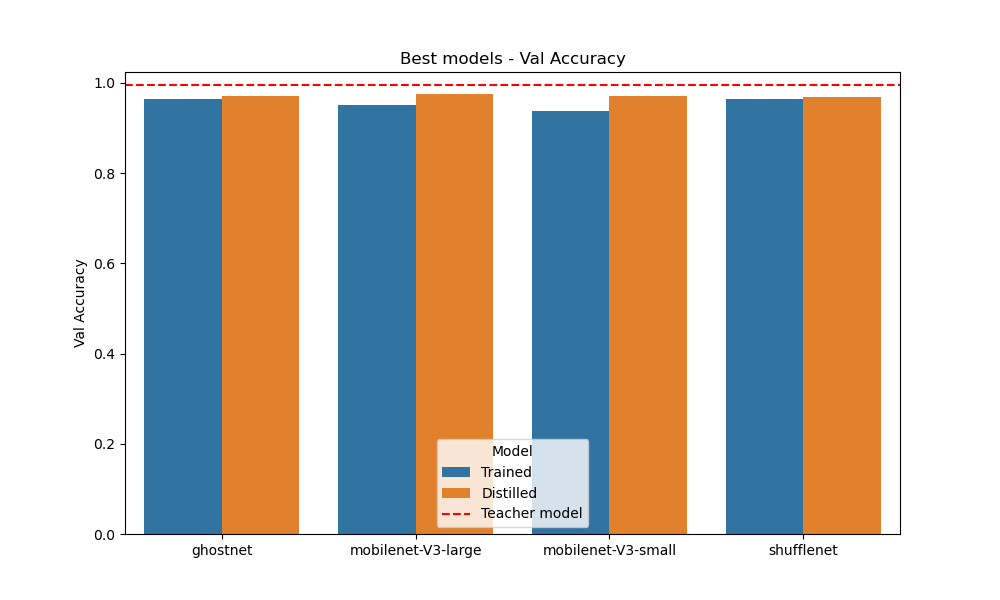
\includegraphics[width=0.9\linewidth]{assets/val accuracy_Best}
	\caption{Validation Accuracy of Different Student Architectures}
	\label{fig:acc_res}
\end{figure}

\section{Results}
Figure \ref{fig:acc_res} depicts the validation accuracy of the teacher model, represented by a red dashed line, along with the best model trained with Knowledge Distillation (KD) and the model trained from scratch for each of the four student architectures. Notably, the validation accuracies of the models trained with KD closely align with that of the teacher model, indicating successful knowledge transfer. They also marginally yet consistently outperform the models trained from scratch for each student architecture. This indicates that all architectures perform comparably well and that KD offers a consistent advantage. The validation accuracy is very close to the teacher for all student architectures, as shown in Figures \ref{fig:val_acc_ghostnet}, \ref{fig:val_acc_mobilenet_large}, \ref{fig:val_acc_mobilenet_small} and \ref{fig:val_acc_shufflenet}.

\begin{figure}[htbp]
	\centering
	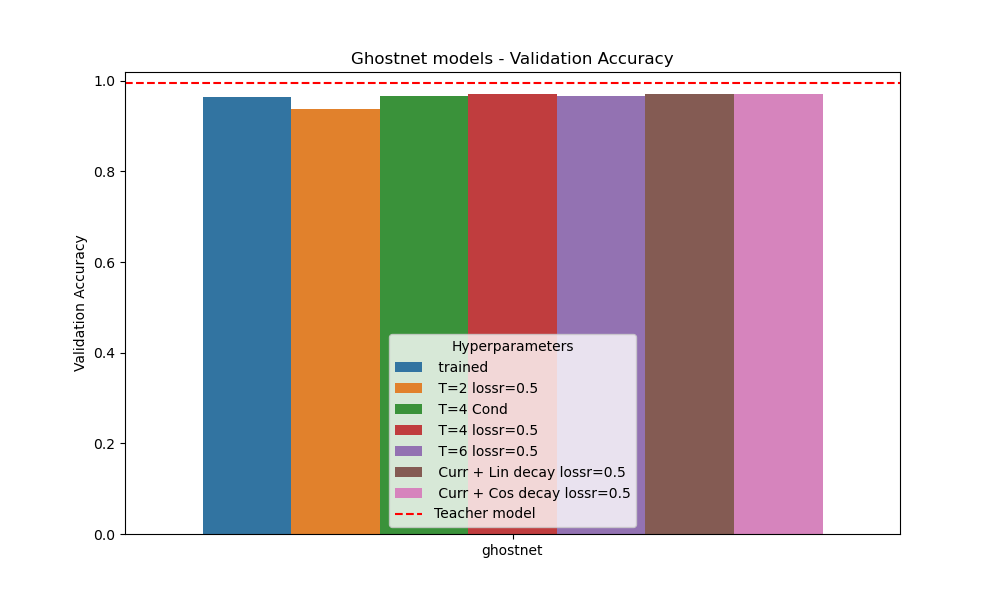
\includegraphics[width=0.9\linewidth]{assets/validation accuracy_ghostnet.png}
	\caption{Validation Accuracy of GhostNet}
	\label{fig:val_acc_ghostnet}
\end{figure}
\begin{figure}[htbp]
	\centering
	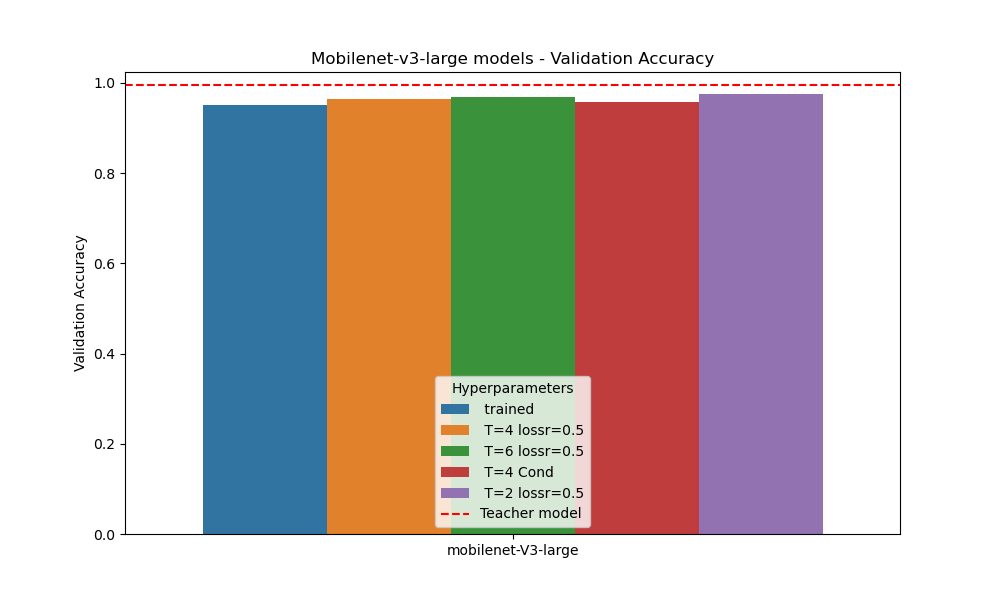
\includegraphics[width=0.9\linewidth]{assets/validation accuracy_mobilenet-V3-large.png}
	\caption{Validation Accuracy of MobileNet V3 Large}
	\label{fig:val_acc_mobilenet_large}
\end{figure}
\begin{figure}[htbp]
	\centering
	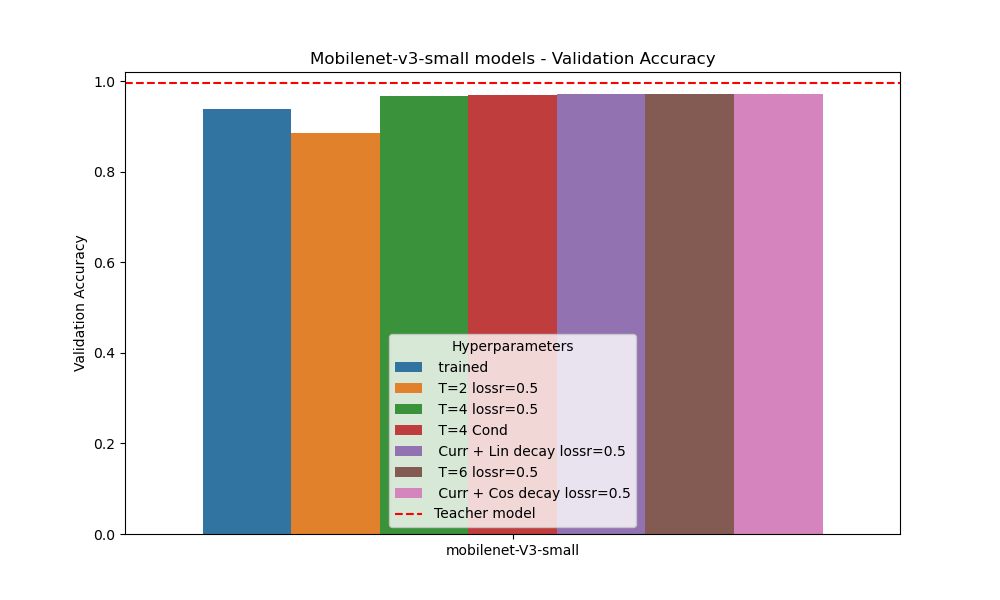
\includegraphics[width=0.9\linewidth]{assets/validation accuracy_mobilenet-V3-small.png}
	\caption{Validation Accuracy of MobileNet V3 Small}
	\label{fig:val_acc_mobilenet_small}
\end{figure}
\begin{figure}[htbp]
	\centering
	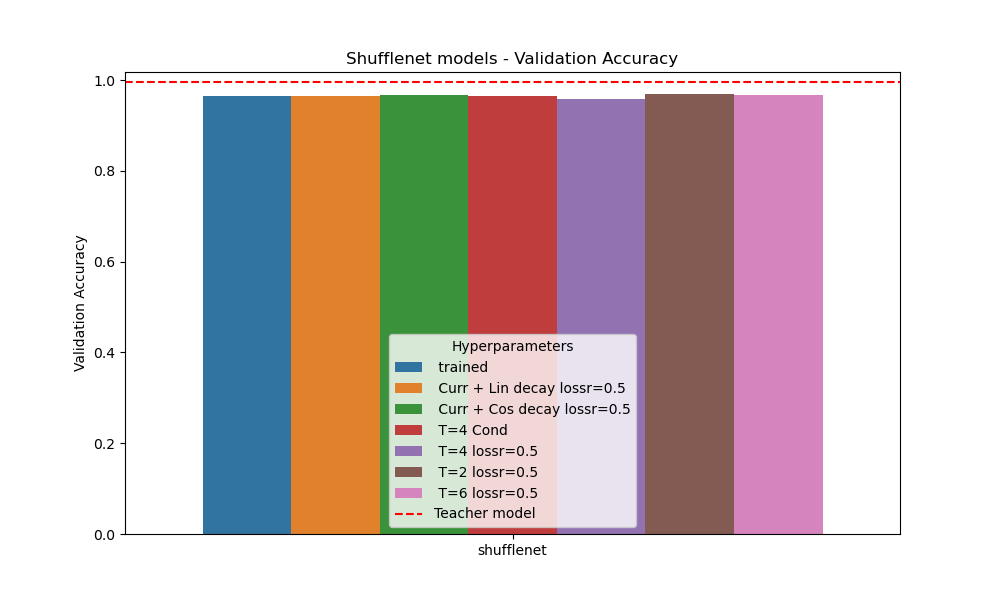
\includegraphics[width=0.9\linewidth]{assets/validation accuracy_shufflenet.png}
	\caption{Validation Accuracy of ShuffleNet}
	\label{fig:val_acc_shufflenet}
\end{figure}

Our experiments revealed distinct optimal hyperparameters for each student architecture. The GhostNet model achieved its best performance using curriculum learning with a linear decay schedule for temperature and a loss rate of 0.5. For the MobileNet V3 Large and ShuffleNet models, optimal performance is obtained with a temperature parameter of 2 and a loss rate of 0.5. On the other hand, the MobileNet V3 Small model performs best when curriculum learning is combined with cosine decay schedule for temperature and a loss rate of 0.5.

\begin{figure}
	\centering
	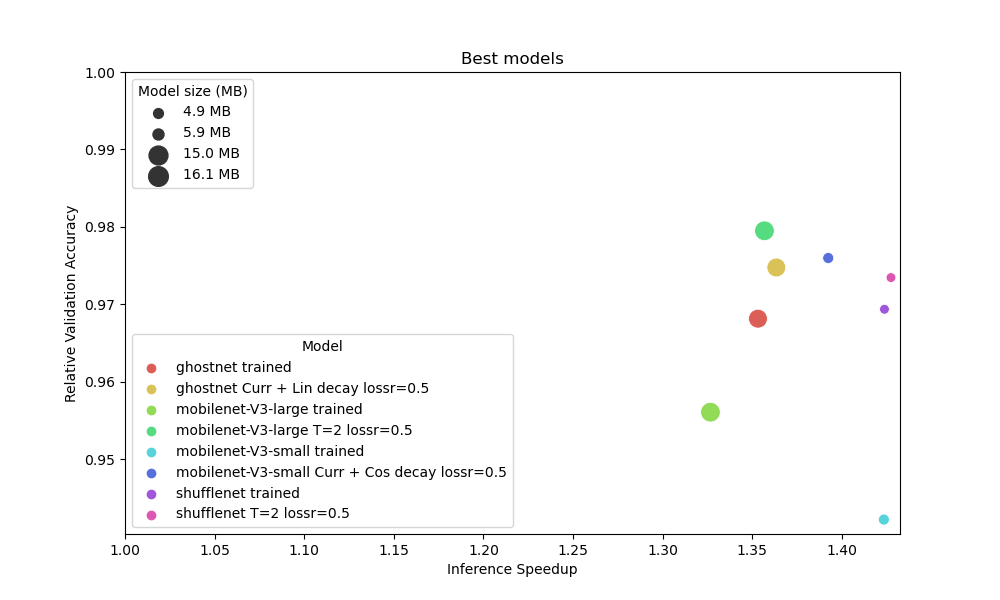
\includegraphics[width=0.9\linewidth]{assets/fat_plot_best}
	\caption{Relative Validation Accuracy and Inference Speedup of Different Student Architectures Trained with KD and from Scratch}
	\label{fig:scatter_res}
\end{figure}

Figure \ref{fig:scatter_res} depicts a scatter plot that illustrates the relative validation accuracy (compared to the teacher model) and inference speedup of each student model, both for models trained with KD and those trained from scratch. The thickness of each point represents the memory footprint of the model in MB.

All student models, when trained with KD, achieved similar performance, with relative validation accuracies ranging from 0.975 to 0.98 and inference speedups between 1.35 and 1.4 times. However, models trained from scratch showed a decrease in accuracy down to 0.95. Interestingly, there are some variations in inference speed even between models with the same architecture which could be attributed to slightly inconsistent allocation of hardware resources or variations in memory management during inference operations. Despite these variations, inference speed is generally close across all architectures.

Among all models, MobileNet V3 Large had the highest relative validation accuracy at 0.98 while MobileNet V3 Small and ShuffleNet achieved slightly higher inference speedups of 1.4 times.

These findings suggest that student models trained with KD not only match the performance of their teacher models but also benefit from faster inference speed and lower memory usage.

\begin{figure}
	\centering
	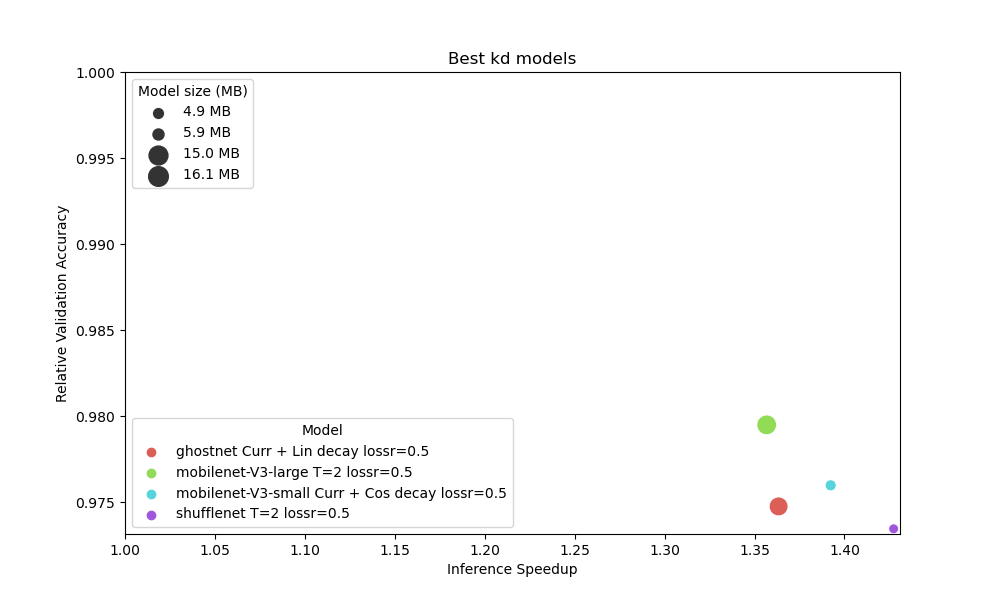
\includegraphics[width=0.9\linewidth]{assets/fat_plot_best KD}
	\caption{Relative Validation Accuracy and Inference Speedup of Different Student Architectures Trained with KD}
	\label{fig:scatter_kd_res}
\end{figure}

Figure \ref{fig:scatter_kd_res} provides a focused view on only those models trained with KD, further emphasizing these observations.


\section{Limitations}
Due to the limited available time for the project and project specific circumstances multiple limitations have to be considered regarding the achieved results. Because of significant training times and the time constraints set by the project course, the search space for different hyperparameter combinations was heavily restricted. With the same reasoning no statistical significance testing was performed and experiments for each setup only performed once. This weighs even more heavy for this project since the student models reach very good results even without knowledge distillation and the different distillation techniques are very close in performance. Therefore, the results can only be interpreted as indications, especially regarding the differences between different knowledge distillation techniques.
For a few experiments a batch size of $ 32 $ was also tested and achieved slightly better results but due to the increased training time with a reduced batch size, this was not further pursued.
The captured data for training and inference speed is very noisy, likely because of the shared nature of the computing resource, therefore for speeds the median batch time or the minimum epoch times are reported.

\newpage
\section*{Acknowledgment}
"The computations were enabled by resources provided by the National Academic Infrastructure for Supercomputing in Sweden (NAISS) at Chalmers e-Commons at Chalmers partially funded by the Swedish Research Council through grant agreement no. 2022-06725."

\bibliographystyle{plain}
\bibliography{bib}

\end{document}

